\documentclass[12pt a4paper]{article}
\renewcommand{\baselinestretch}{1.5} 

\usepackage[T1]{fontenc}
\usepackage[utf8]{inputenc}

\usepackage{graphicx}
\usepackage{geometry}
\usepackage{subcaption}

\usepackage{mathtools}
\usepackage{amsmath}

\usepackage{hhline}
\usepackage{multirow}
\usepackage[table,xcdraw]{xcolor}
\usepackage{float}
\usepackage{array}
\usepackage{hyperref}
\usepackage{titlesec}
\usepackage[super]{nth}

\usepackage{physics}

\usepackage[toc,page]{appendix}

\renewcommand{\baselinestretch}{1.5}
\newcommand\qtageq{\stackrel{\mathclap{\normalfont\mbox{?}}}{=}}
\newcommand\exclmeq{\stackrel{\mathclap{\normalfont\mbox{!}}}{=}}

\geometry{
 a4paper,
 left= 2.2cm,
 right = 2.2cm,
 top = 2.2cm,
 bottom = 2.2cm 
 }


\titleformat
{\subsubsection} 
[display] 
{\itshape \bfseries \large} 
{} 
{-5ex}
{
    \vspace{0ex}
}
[
\vspace{0ex}
] 


\newcolumntype{?}{!{\vrule width 2pt}}
\numberwithin{equation}{section}

\begin{document}
\thispagestyle{empty}
\begin{titlepage}
\title{Cats \& Dogs audio classification \\ Project report}  
\author{Portik Attila, BKF0JP}
\end{titlepage}
\maketitle


\section{Introduction}
The "cats and dogs" image dataset is one of the best known and most commonly used example for the classification, and therefore, we already know loads of accurate methods for solving that classification problem.  For me, the most impressive result of machine learning and deep learning is that we are able to create algorithms that can recognize and identify new information based on their earlier experience. I have previously worked on an image classification task, therefore I wanted to make my project a little more interesting. That is why I chose the audio classification, and I found the audio classification version of the cats and dogs image classification problem, as a Kaggle dataset. (see ~\cite{data})


The chosen dataset consists of audio files in "wav" format, and any of these contains dog barking or cat's meow. At first sight, the usability of the dataset was questionable because the data set contains relatively little data, the length of the audio strings is very varied, there are a few poor quality recordings, and the dataset is unbalanced. Examination of the data set shows that there are indeed problems that make classification difficult. But by preprocessing the data and choosing the proper features, they have been solved and achieved relatively well accuracy. 

\section{The dataset}

The chosen dataset contains at all 277 audio files at all, in wav format. The .wav files are used for storing uncompressed audio bit-streams. By checking the database soon revealed that some of the files were completely unusable, which I removed. Here the unusable samples do not mean the noisy poor-quality recordings or which contains other sounds (like human speech). I use these recordings since the sound-recognizing in the presence of ambient noise is considered as the part of the task. The problem was that there were audio files with completely different content. I found and removed ten such files from the data set. That solved the first part of the problem. The other big issue was that the data set contained far more samples from cats than from dogs. However, the data set does not contain too many samples, so it was not possible to easily balance it by omitting some samples. I was able to find another dataset that contains recorded dog barking (see ~\cite{data2}).  Adding these to the original data set, I get two classes of roughly the same size (see FIG. ~\ref{fig1}). 

\begin{figure}[H]
\centering
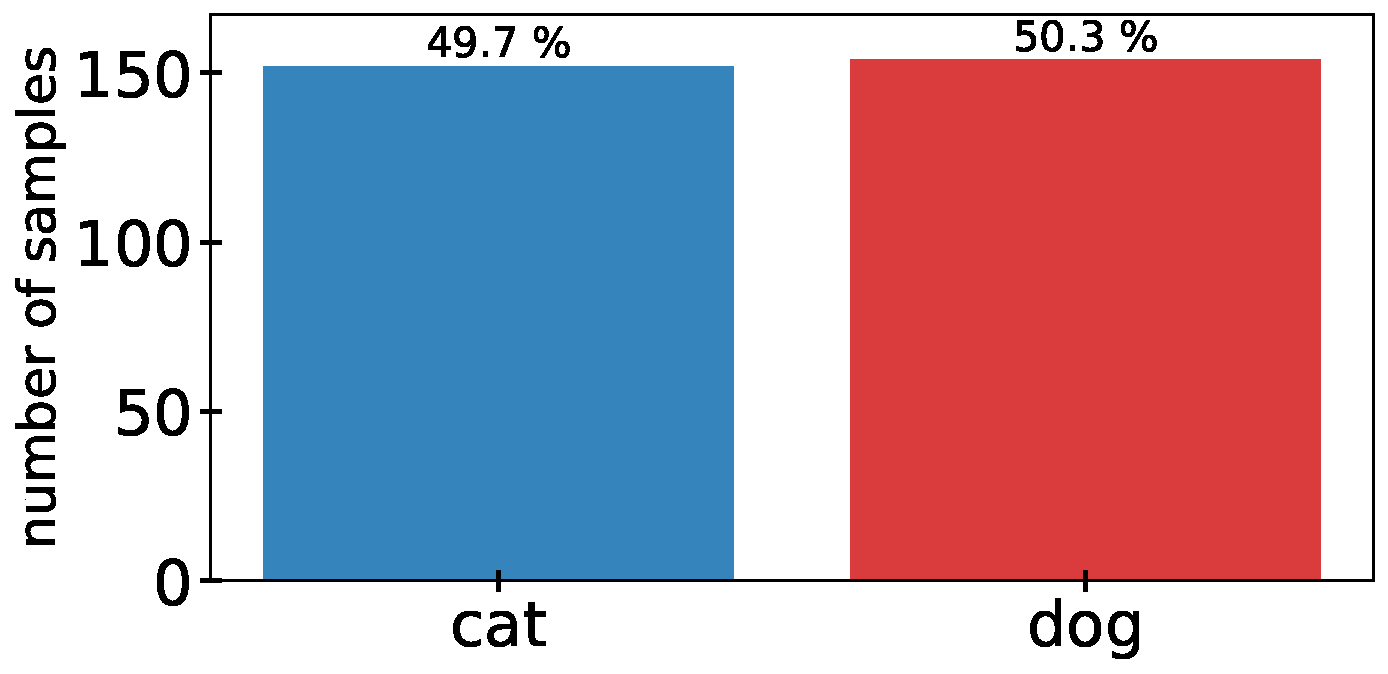
\includegraphics[width=0.8\textwidth]{fig/ration.pdf}
\caption{The distribution of the samples in the two classes.}
\label{fig1}
\end{figure}

I used the SciPy (scipy.io.wavfile.read) python package to load the audio files and create NumPy arrays from those. This loads any raw audio files in which data is stored as pulse-code modulation values. As the input, we get the time series of the amplitudes and sampling rate of the .wav file. Two random examples for the sampled signal are shown in figure ~\ref{fig2}.

\begin{figure}[H]
\centering
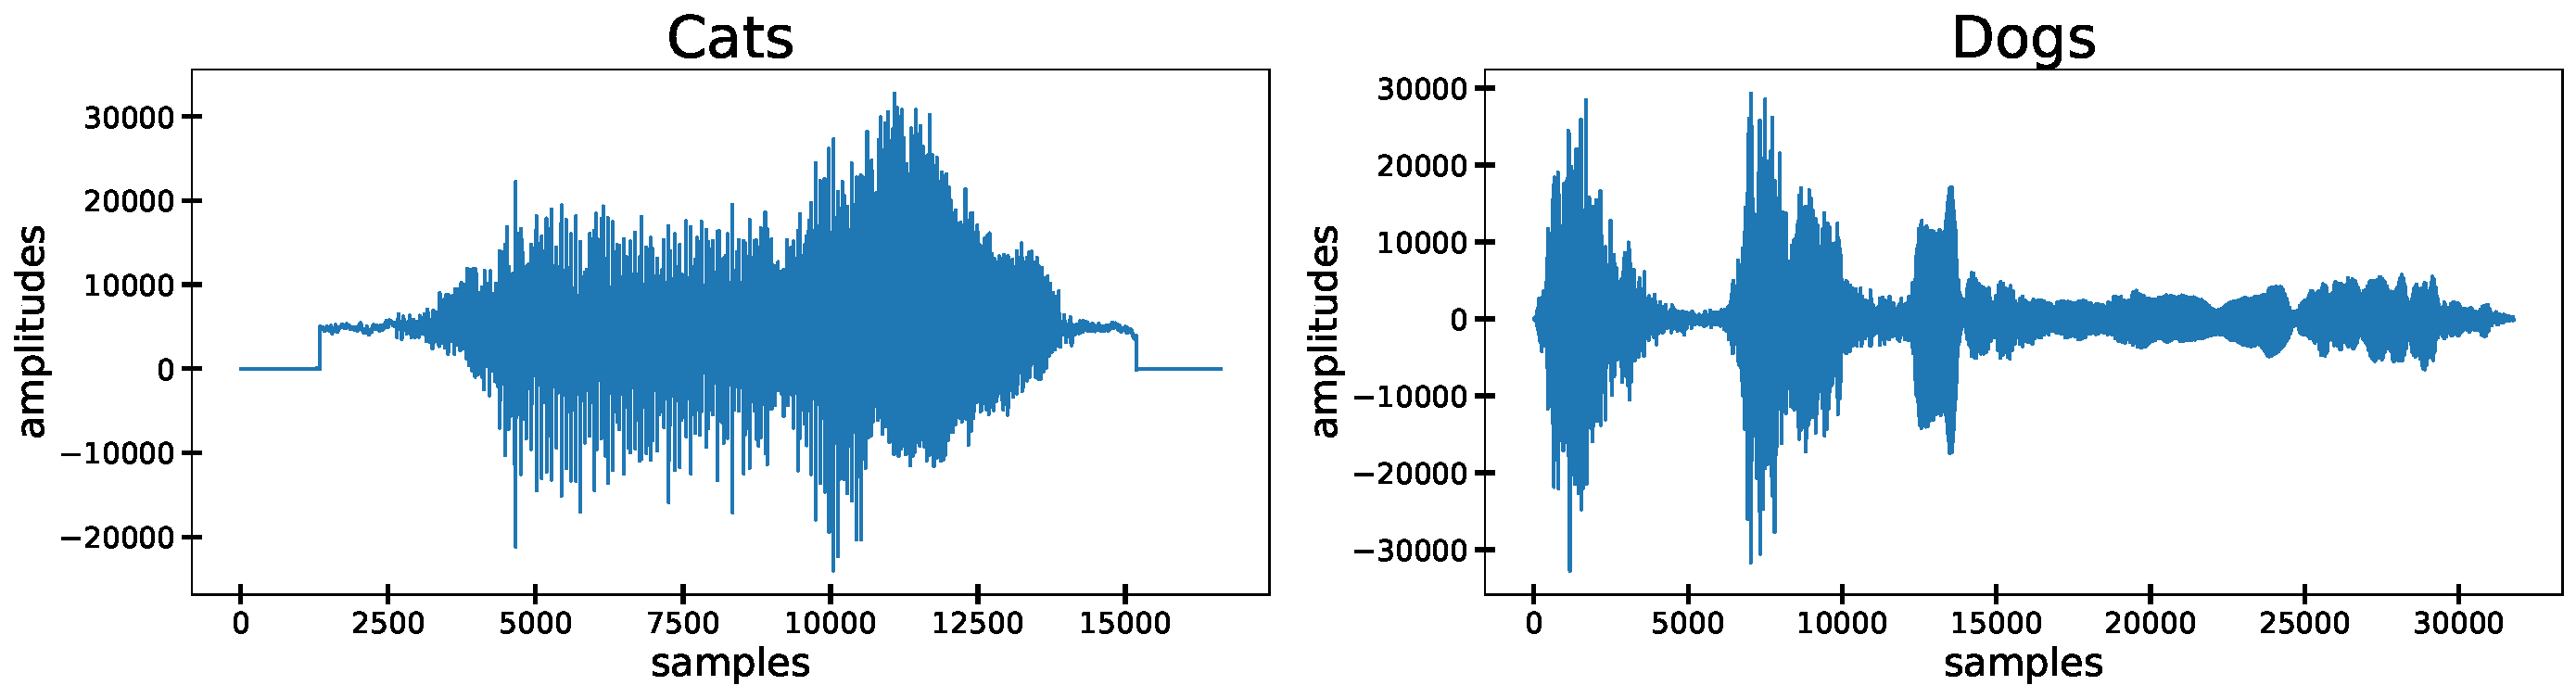
\includegraphics[width=0.99\textwidth]{fig/example.pdf}
\caption{Example audio sample from cats (left) and dogs(right).}
\label{fig2}
\end{figure}
It is not possible to determine by the naked eye which sample belongs to which class. In the following figure, I have shown all the samples from each class (see FIG. ~\ref{fig3}). There, one already can observe certain characteristics of the two classes. But it is not yet possible to decide on a sample where it belongs.

\begin{figure}[H]
\centering
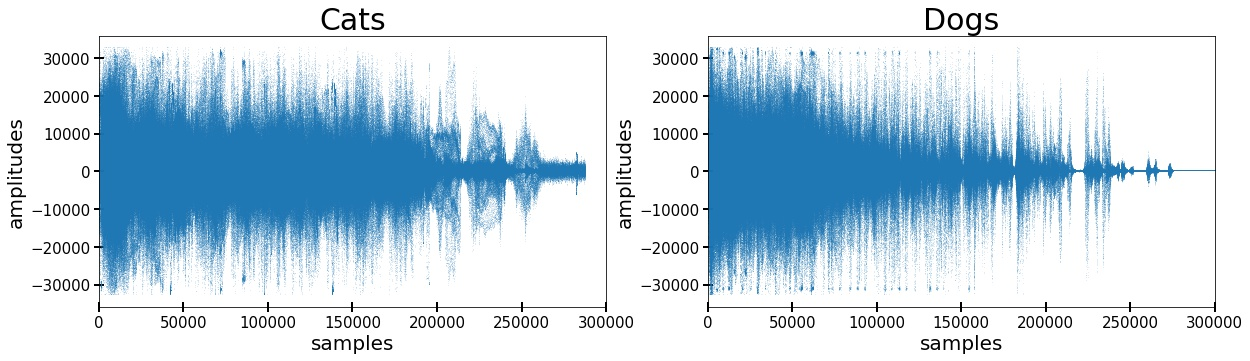
\includegraphics[width=0.99\textwidth]{fig/all.jpg}
\caption{The common part of the samples for the two classes.}
\label{fig3}
\end{figure}

The last difficulty with the dataset is the variety of the lengths of its elements. A common trick in audio classification is the segmentation of the samples. In this way, more samples of the same length can be formed from one sample.  But this is not suitable for this dataset, since a segment of the sample does not contain the required information for the classification. In contrast, in the music classification, the properties of the sample can be determined based on a short part of the sample. In the current task, one can solve the mentioned problem by choosing the proper features and classification methods.

\section{Features}

A commonly used method in audio classification is to calculate the spectrum of audio samples. Then one can train convolutional neural networks on the spectra as image-like data, thus creating a model that can perform the classification. The problem is that, as I mentioned above, the samples in the given dataset are not equal in length thus the spectra would not be equal in size.  One way to solve the problem is to take the time average of the spectra as features. At the same time, this solution, give the opportunity to use other machine learning methods instead of convolutional neural networks. In the next part, I will present the features that I used for the classification. I tried to choose properties of the samples that are significantly different for the two classes so that the classification can be done based on them. To manage the audio data and calculate its properties, I used the functions of librosa, which is a python package for music and audio analysis. The python notebook that contains the codes is available at this GitHub repository: \cite{repo}.
 
\subsection{The mel-spectrogram}

The most important features come from the mean values of the mel-frequency cepstral coefficients. The mel-frequency cepstral coefficients collectively make up the mel-frequency cepstrum (a cepstrum is a spectrum of the logarithm of the spectrum of the time signal), which is a representation of the short-term power spectrum of a sound, based on a linear cosine transform of a log power spectrum on a non-linear mel scale of frequency. The motivation of the usage of the mel scale is in that how the hearing works.  Humans perceive sound logarithmically, thus, the mel scale was introduced. It is a logarithmic scale based on the principle that equal distances on the scale have the same perceptual distance. The following figure presents a typical mel spectrogram for each class (see FIG. ~\ref{fig4}). On these, it is obvious the difference between the two types of sound, this suggests that the mel diagram will have a crucial role in the classification.

\begin{figure}[H]
\centering
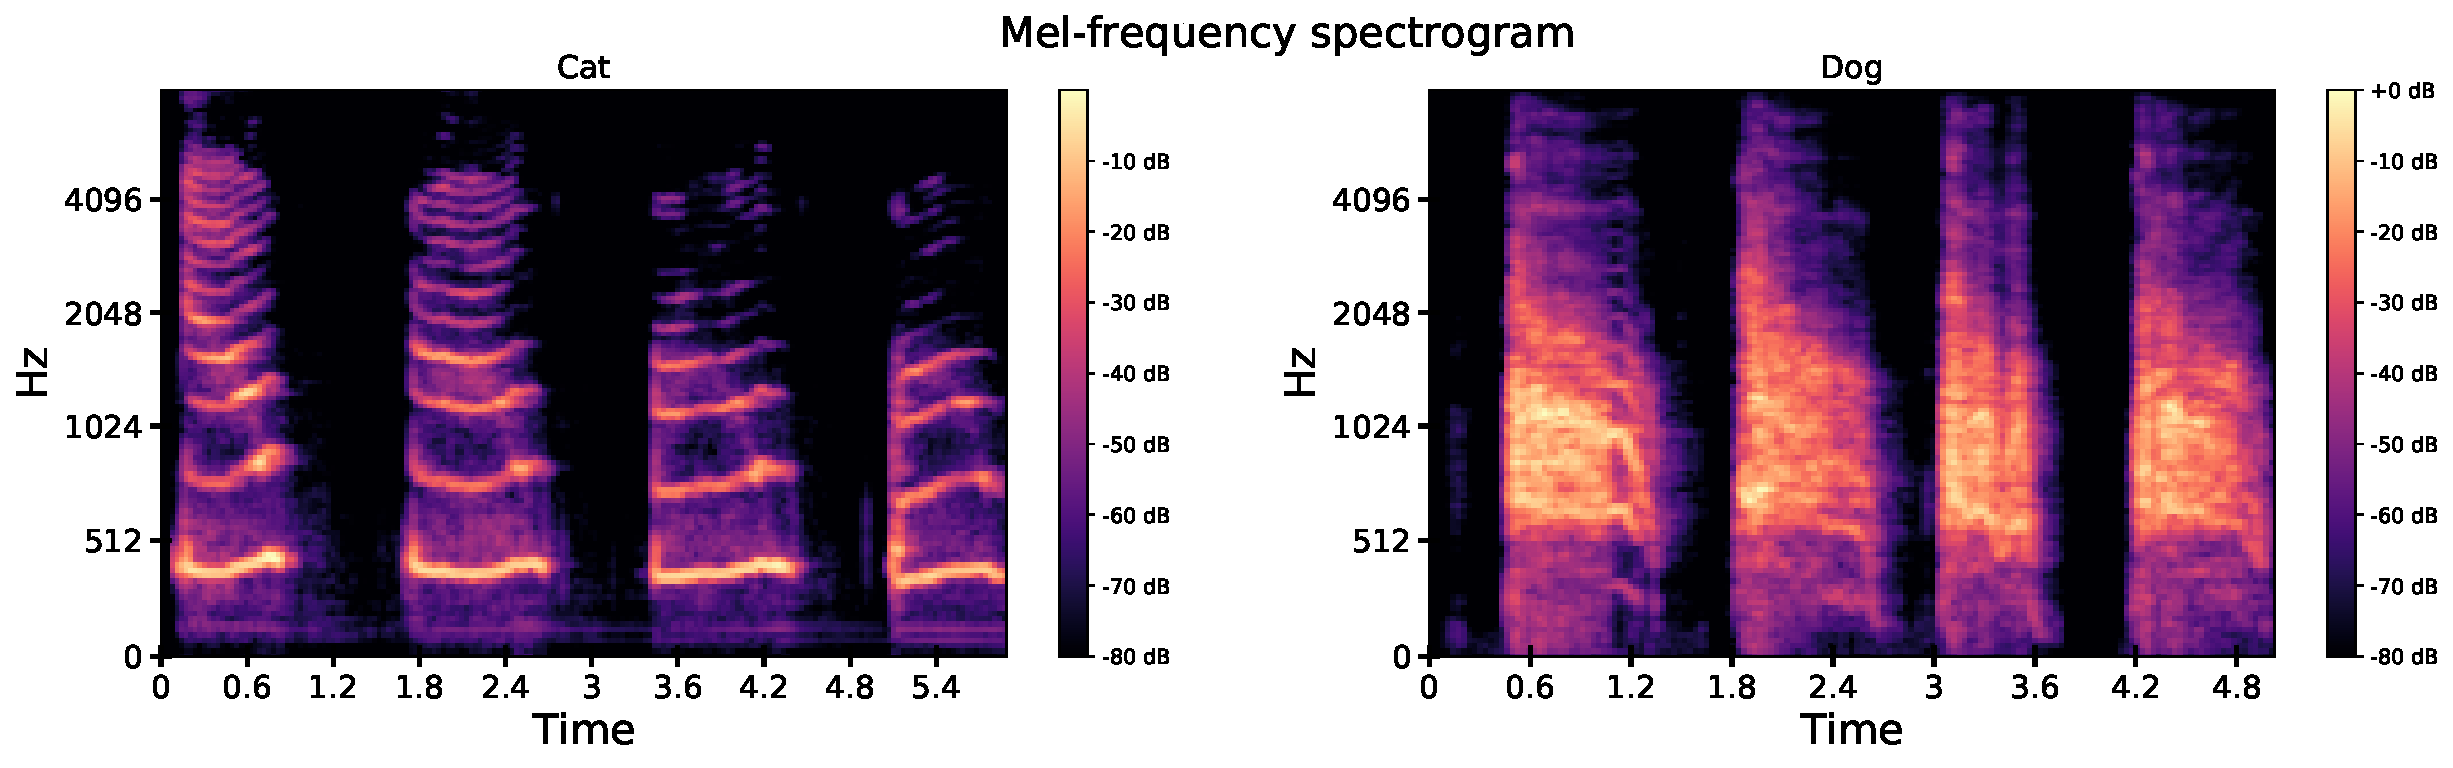
\includegraphics[width=0.99\textwidth]{fig/mel.pdf}
\caption{Typical mel spectrograms for each class.}
\label{fig4}
\end{figure}
Cased, the mentioned problems we can not use directly the mel-spectrograms, but their time average (see FIG. ~\ref{fig5}).

\begin{figure}[H]
\centering
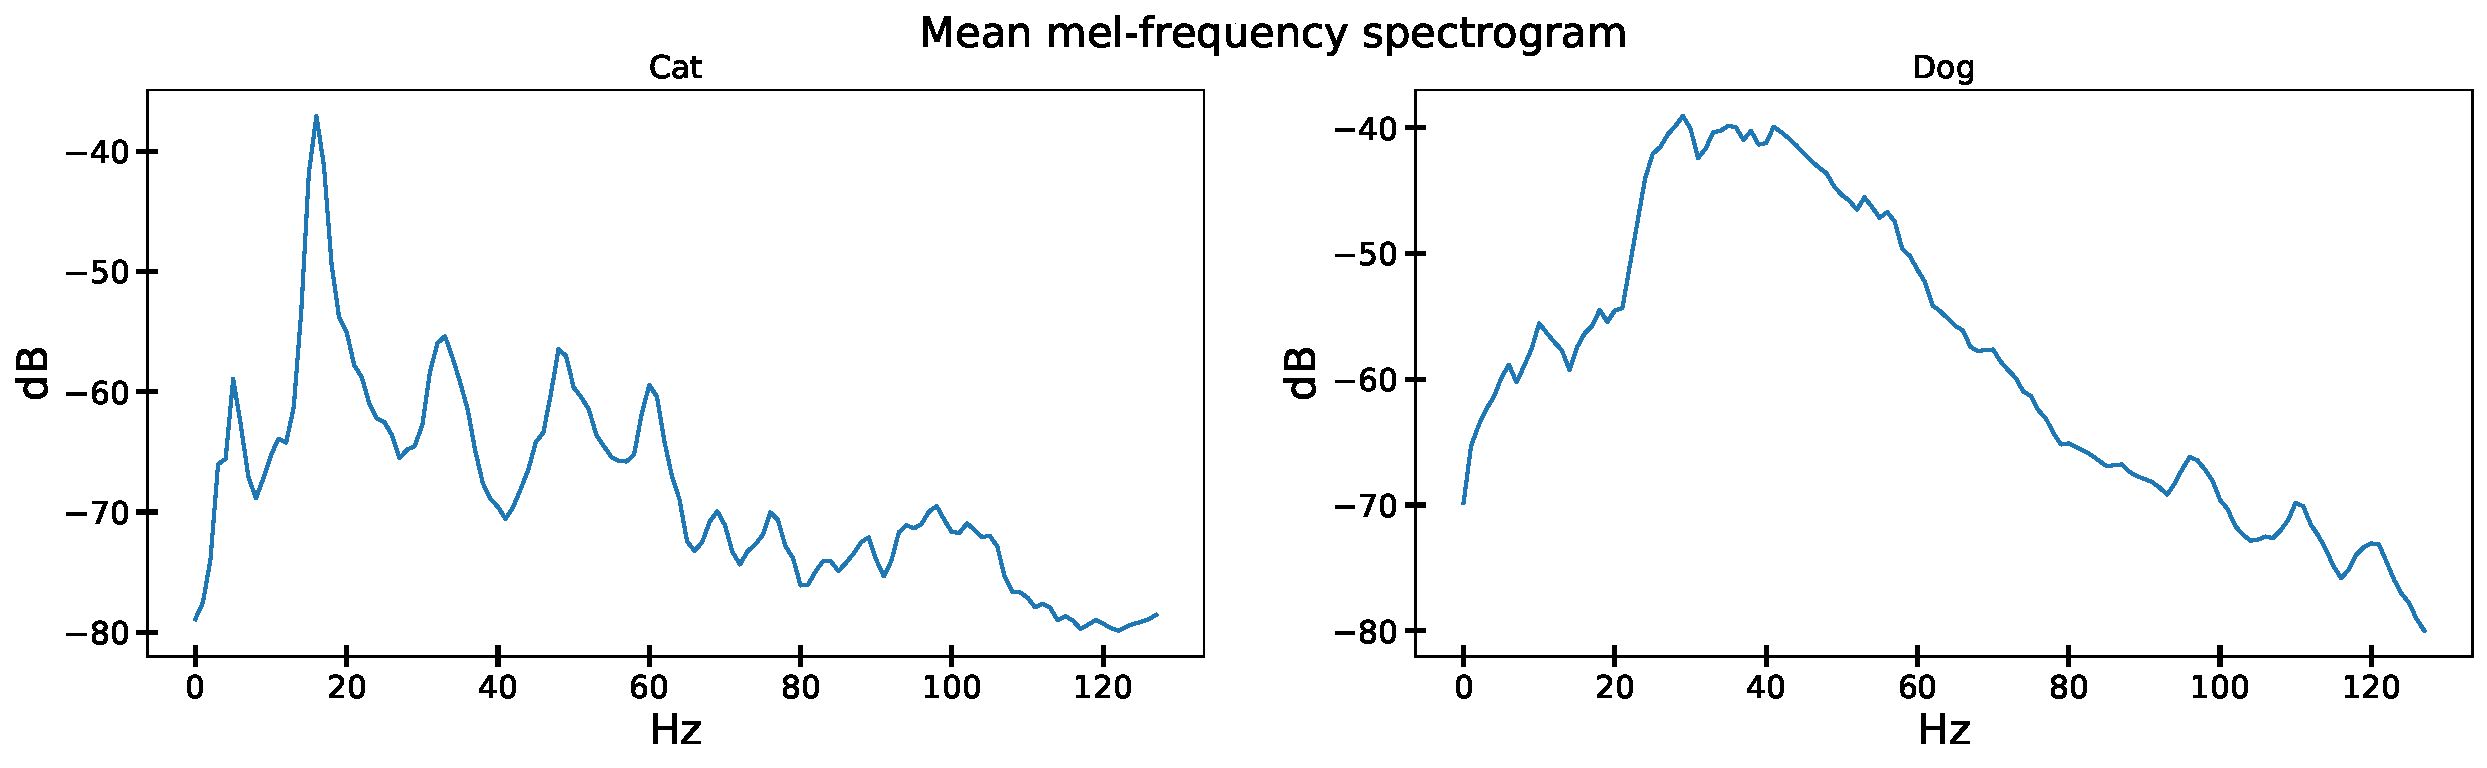
\includegraphics[width=0.99\textwidth]{fig/mel_pro.pdf}
\caption{Typical mean of mel-spectrogram.}
\label{fig5}
\end{figure}

\subsection{The tempogram and tempo}

The next feature is the mean tempogram (see FIG. ~\ref{fig6}).  The tempogram is similar to a spectrogram, it is the time-tempo (beats per minute) representation for a given time-dependent signal. As previously, we first calculate the tempogram, then take its time average. The global tempo of the signal also can be estimated via libros, thus I try to use it as a feature.

\begin{figure}[H]
\centering
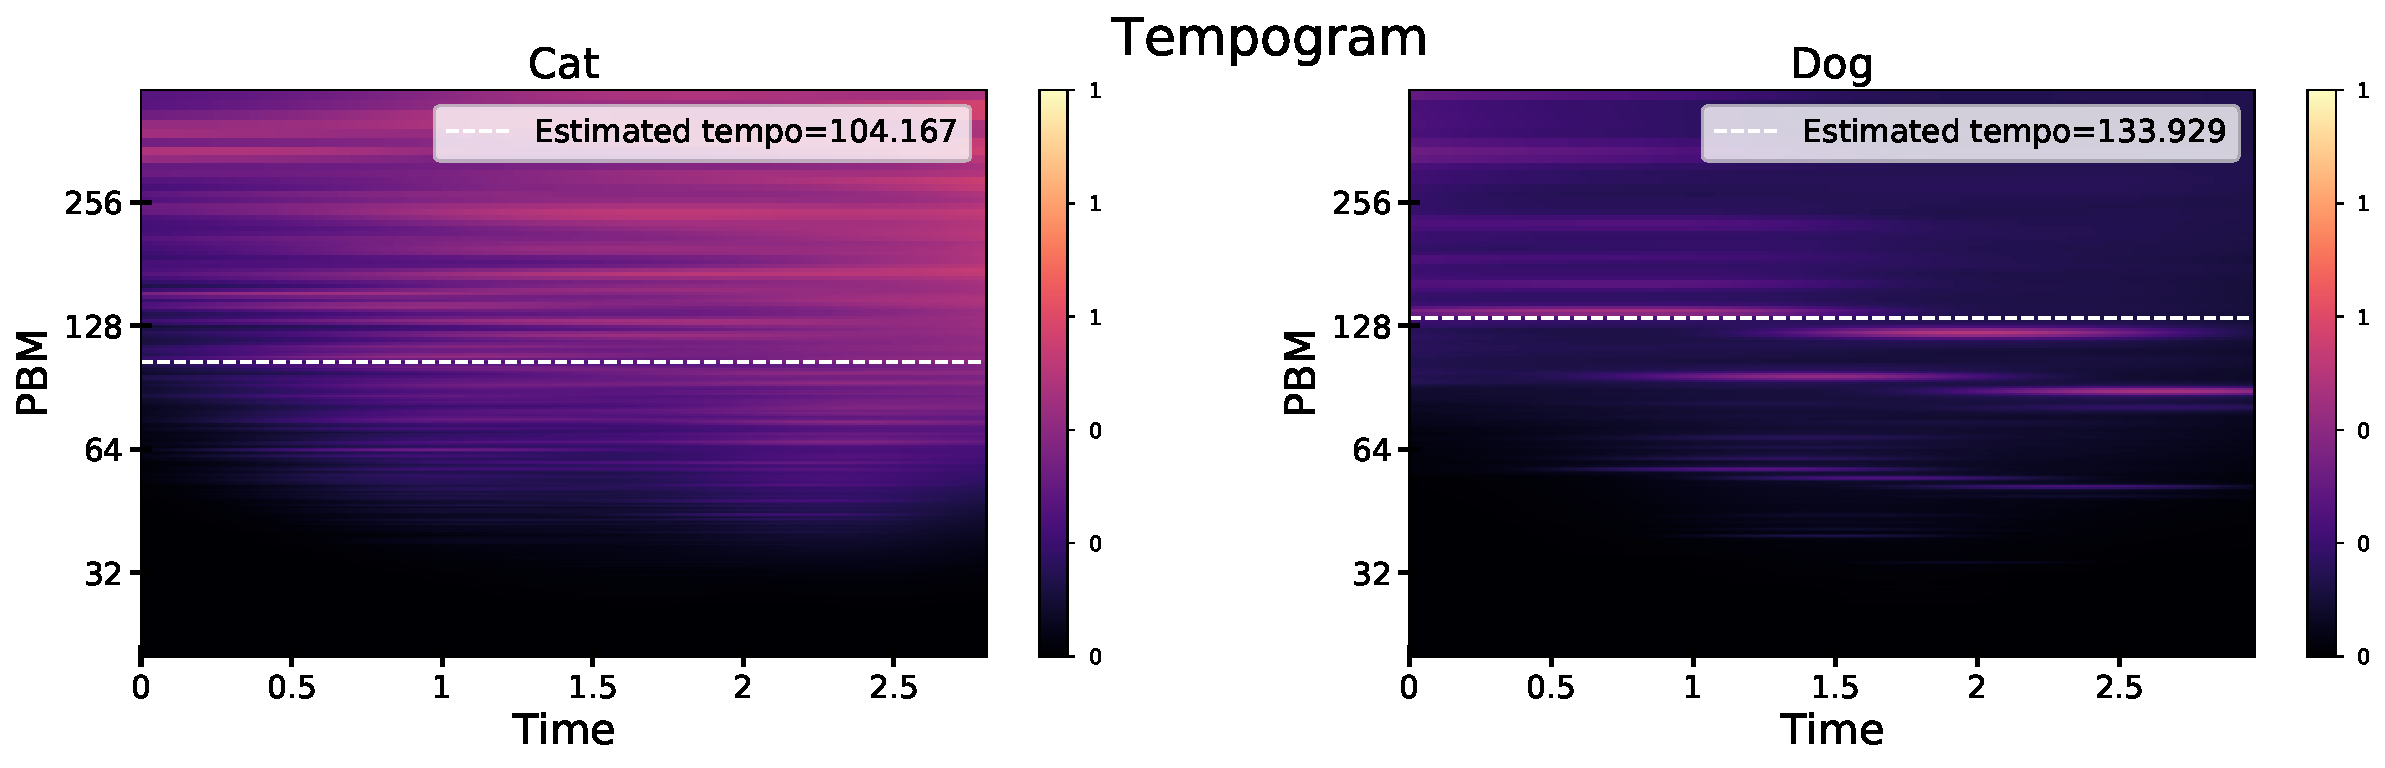
\includegraphics[width=0.99\textwidth]{fig/tempogram.pdf}
\caption{Typical tempograms for each class.}
\label{fig6}
\end{figure}

\subsection{The spectral centroid and bandwidth}

The Spectral Centroid is the centre of gravity of the magnitude spectrum. It defines the frequency band where most of the energy is concentrated. The spectral bandwidth is the variance from the spectral centroid. It marks the spectral range of interest around the centroid(see FIG. ~\ref{fig7}). 

\begin{figure}[H]
\centering
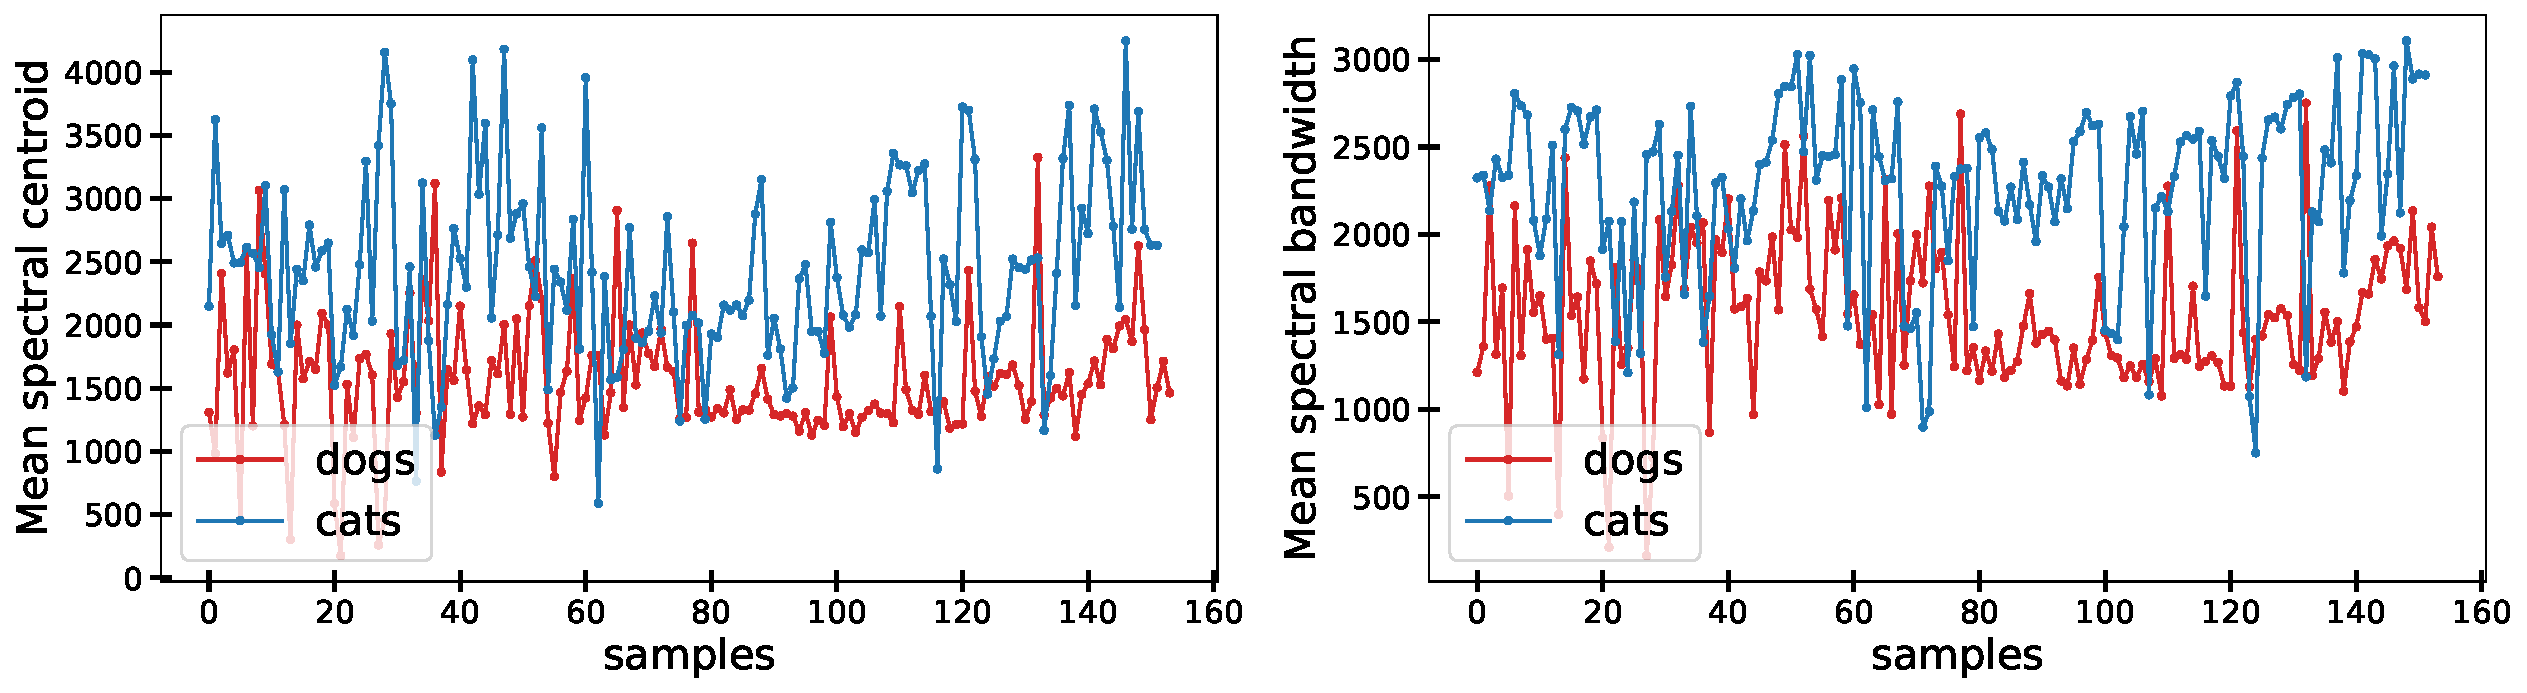
\includegraphics[width=0.99\textwidth]{fig/cen_band.pdf}
\caption{The mean spectral centroid and bandwidth for all samples in the dataset.}
\label{fig7}
\end{figure}

\subsection{The zero-crossing rate and the root mean square energy}

The zero-crossing rate is one of the most basic, commonly used features of the audio samples. It is simply the number of times a waveform crosses the horizontal time axis. Root Mean Square Energy ( the square root of the mean square energy ) is based on all samples in a frame. Higher energy corresponds to a louder sound, it is an indicator of loudness, hence. 

\begin{figure}[H]
\centering
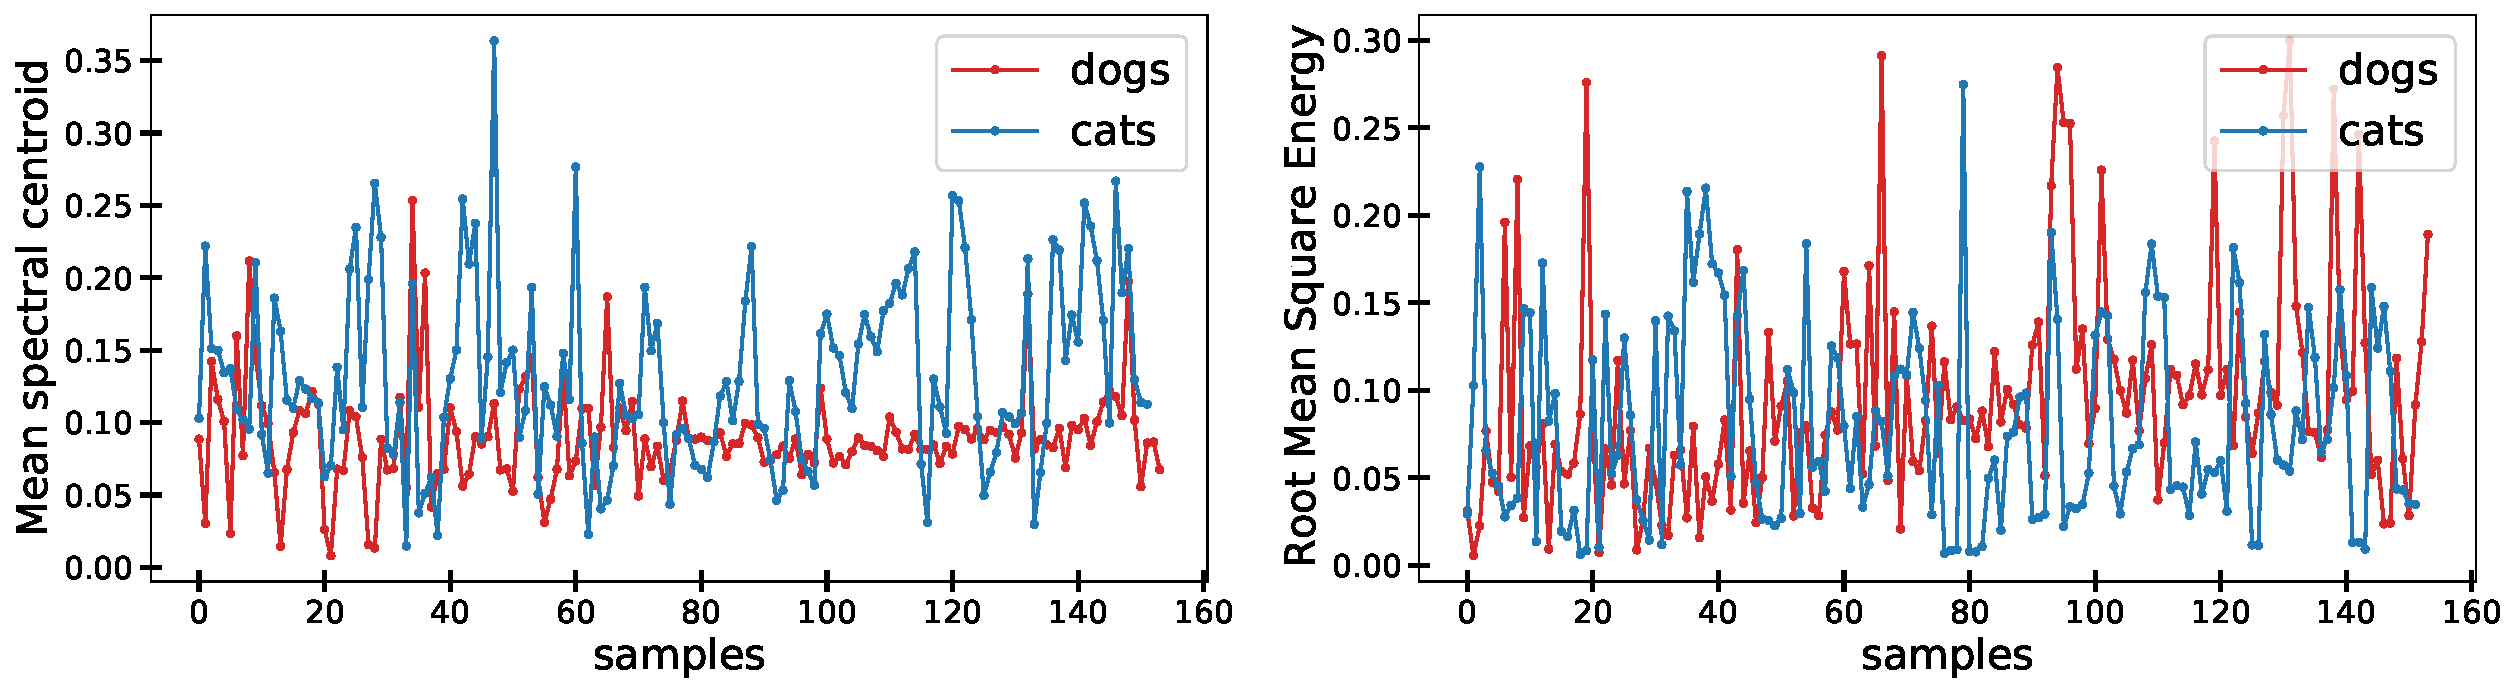
\includegraphics[width=0.99\textwidth]{fig/zer_root.pdf}
\caption{The zero-crossing rate and the mean root mean square energy for both class.}
\label{fig8}
\end{figure}


To accomplish the classification task, I used the enumerated features. There are seven different feature types, these mean 261 features at all (the image like features has 128 components).

\section{Classification}

Because this is a relatively small dataset for binary classification, I am able to try a variety of classification methods. Therefore,  I applied all the suitable methods that made part of the course. And I am going to present the models, which give the highest accuracy. The original dataset makes part of a kaggle event, where the best accuracy of the submitted results is about 90 \%. Therefore, my goal is at least to reach that accuracy. For compactness, I will not present the theoretical background of the models since that has happened during the semester. For the classification, I used a 0.8/0.2 train-test split, and standard scaling and normalization where it is required.

\subsection{Decision tree and random forest classifier}

First, I tried the random forest and decision tree models. I personally like these models, because both instantly give some impression about the importance of the different features. The visualization of the first layers of the tree and the most important features are in figure \ref{fig9}.

\begin{figure}[H]
\centering
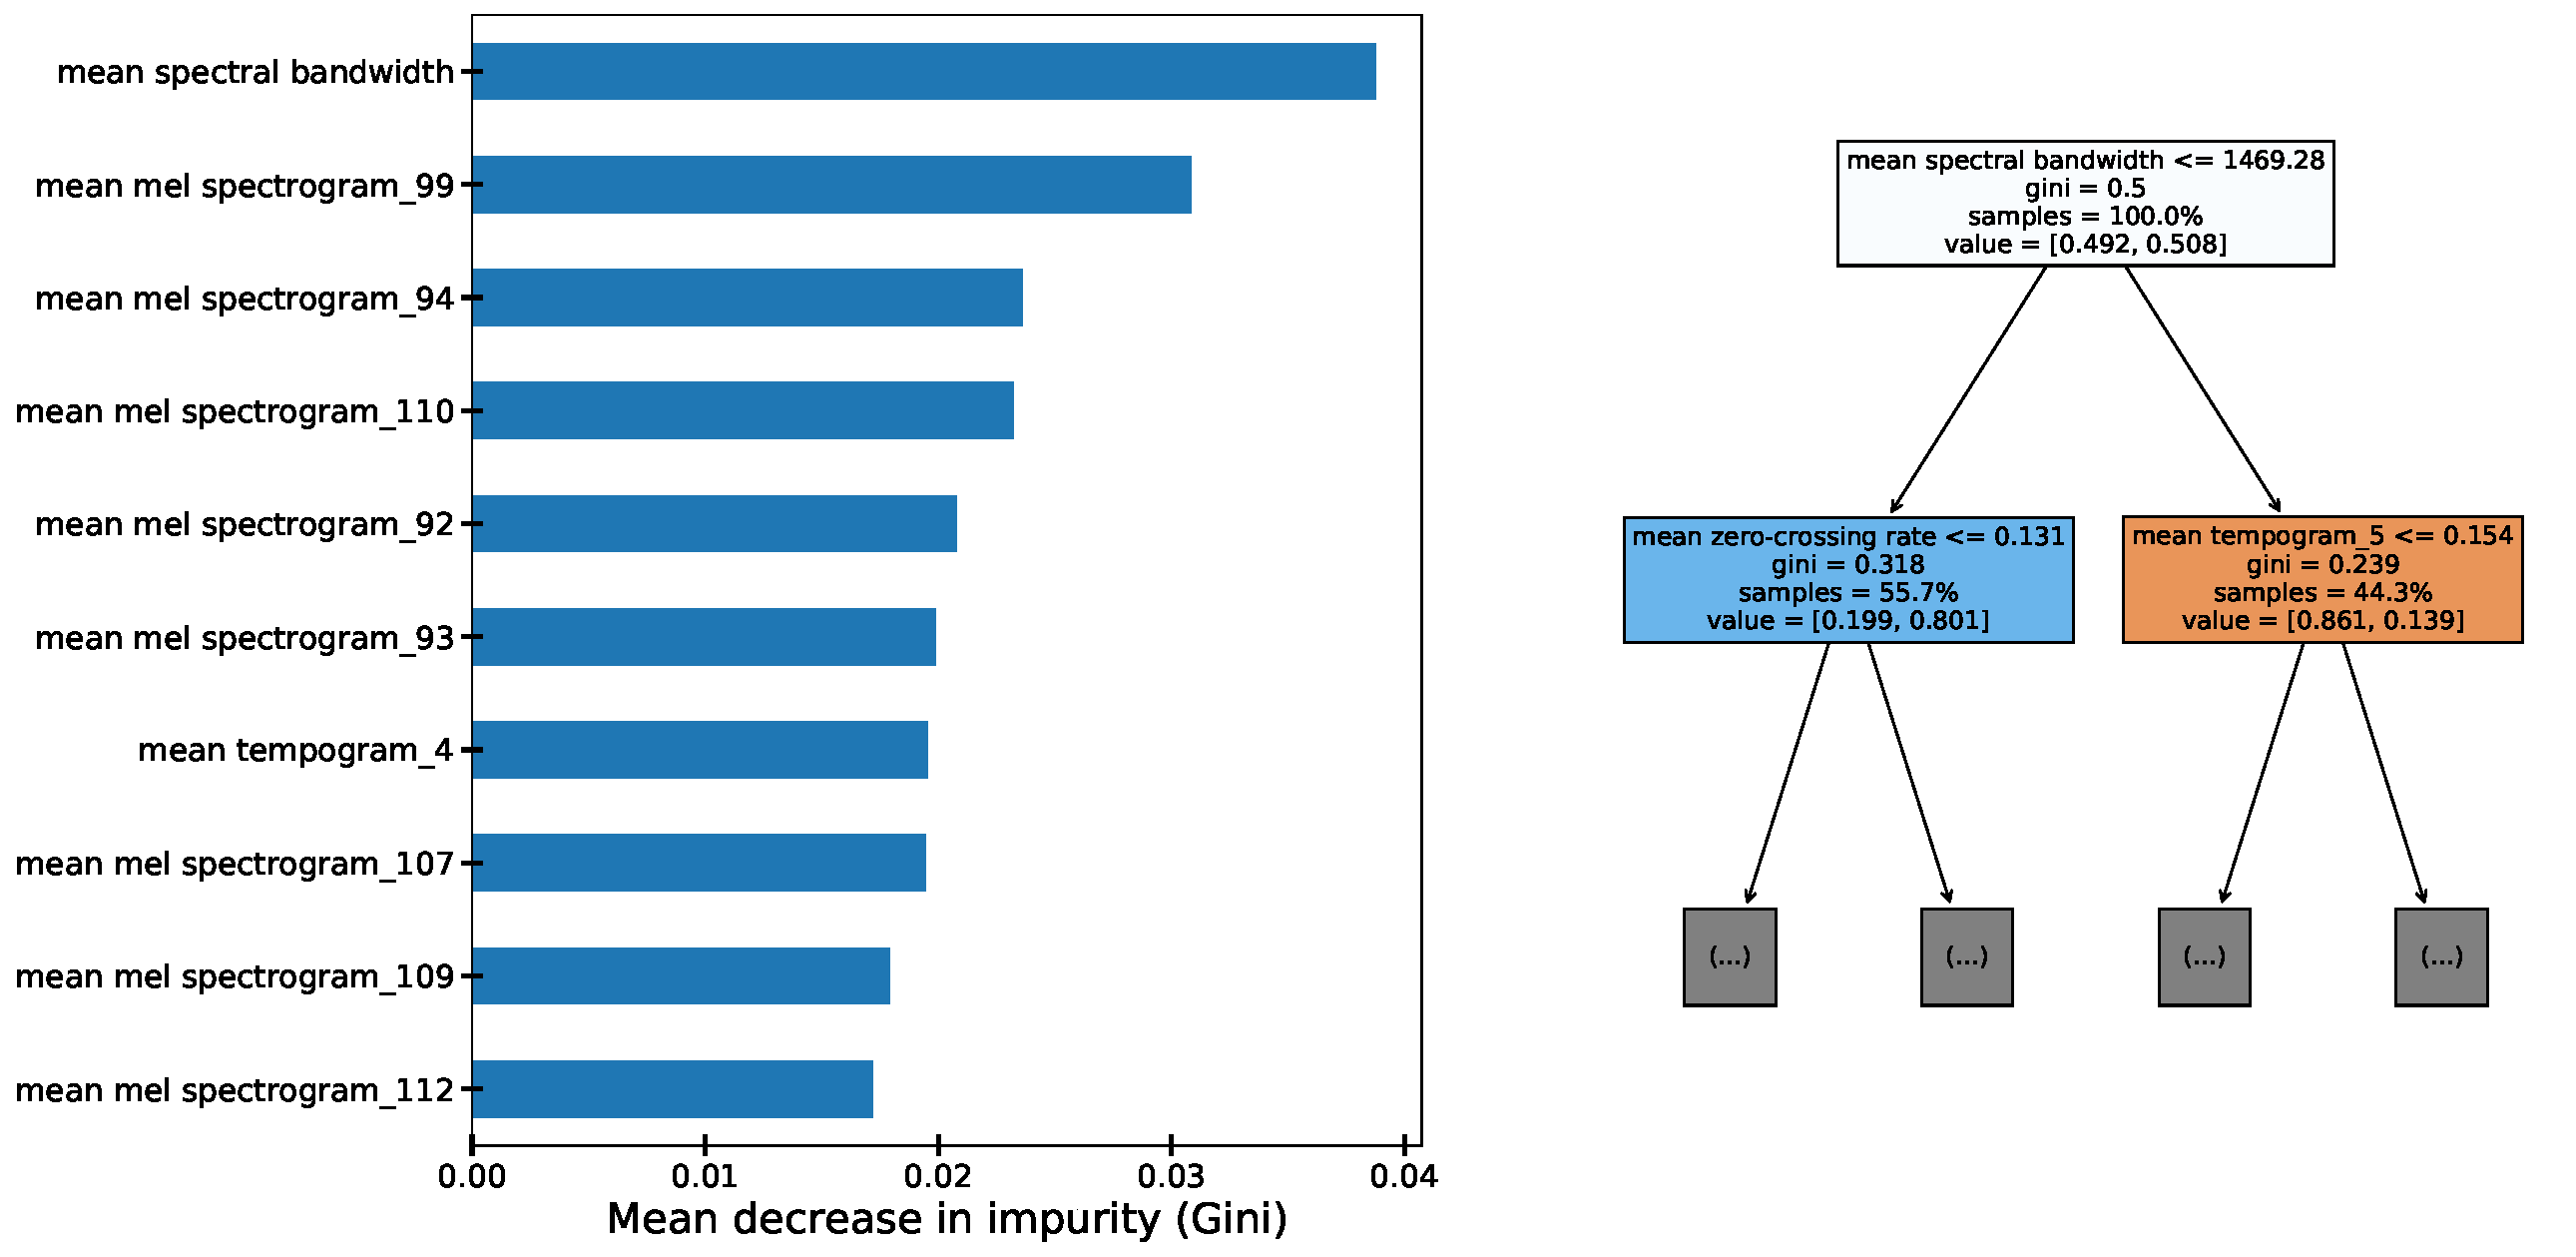
\includegraphics[width=0.99\textwidth]{fig/features.pdf}
\caption{The most important features for random forest classifier (left) and first 2 layers of the decision tree classifier.}
\label{fig9}
\end{figure}
As we expected based on the visualisation, the most features are the spectral bandwidth and the elements of the mel spectrogram. If we look at the figures in the previous section, it is clear that these features contain crucial information from the viewpoint of the classification.


For binary classification, the confusion matrix well describes the accuracy of the model (see FIG.  \ref{fig10}).

\begin{figure}[H]
\centering
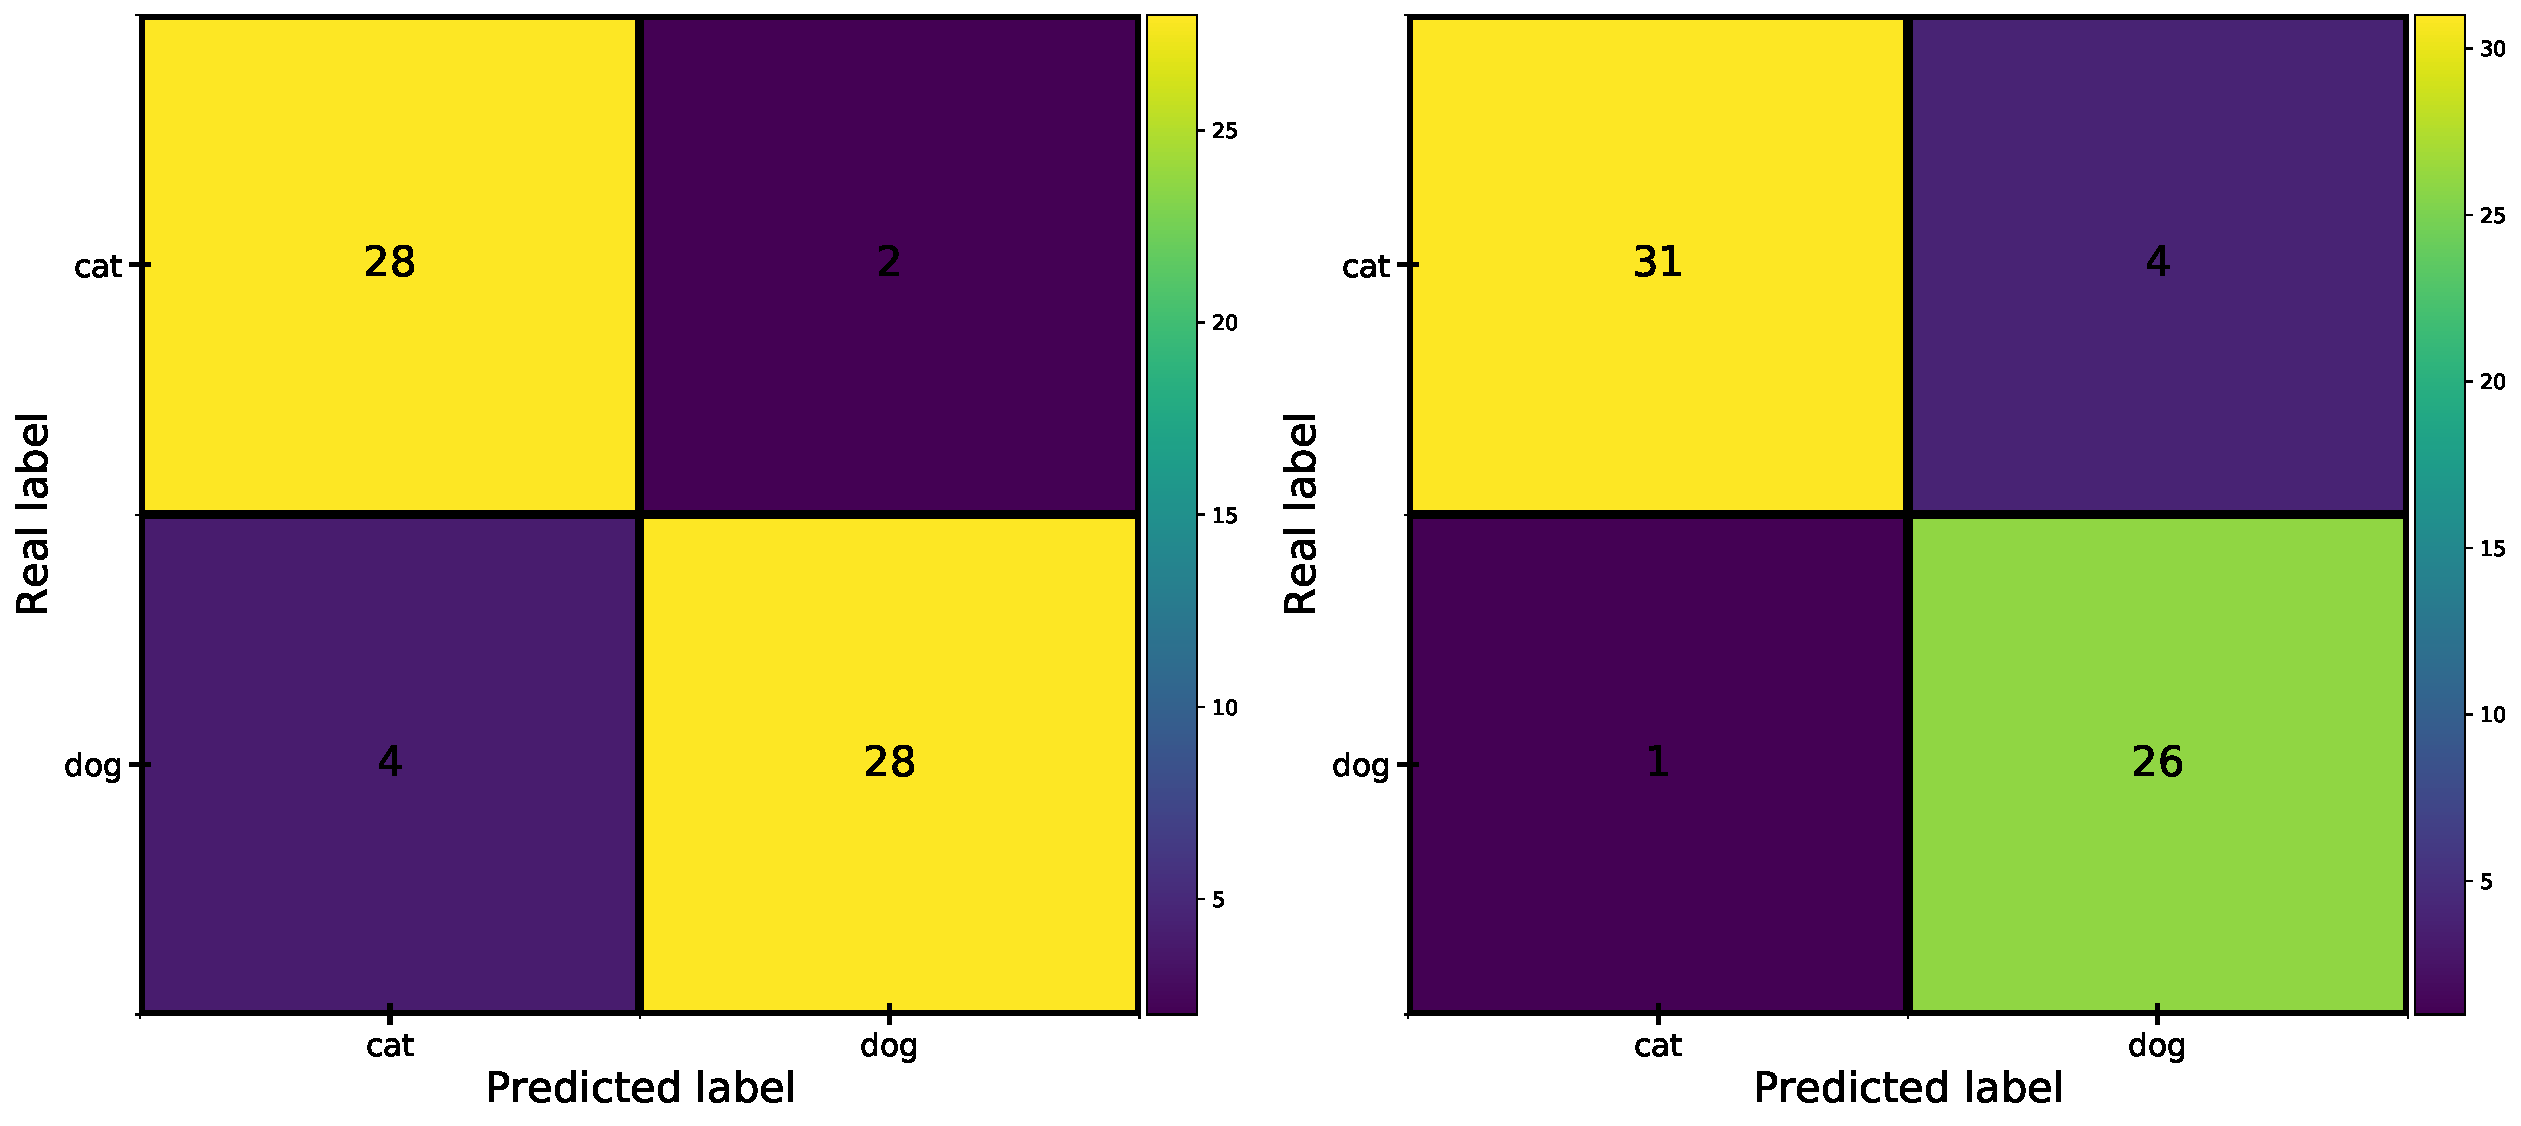
\includegraphics[width=0.7\textwidth]{fig/conf1.pdf}
\caption{The confusion matrix of the predicted class by the decision tree classifier (left) and by the random forest classifier (right). I used both classifiers with the default parameters.   In the case of the decision tree, the accuracy was 90.32 \%. And in the case of the random forest, the test accuracy was 93.55 \%.}
\label{fig10}
\end{figure}

\section{Fully connected neural networks}

Besides the classical learning algorithms, I tried to train a fully connected neural network to classify the dataset. We have a small dataset with a few important features. Therefore we do not need many neurons.  But from the experiences with SVM classifiers (their accuracy was not high enough to present in the report), one can conclude that the decision boundary is not linear.  We need at least two hidden layers, hence. In the case of binary classification, binary cross-entropy is a good choice for loss, and the Adam optimizer is good for that kind of dataset. These were my basic assumption to create a neural network then I defined the concrete parameters by trying out different options. In the end, I found a very small model that can reach higher than 90 \% accuracy.  This builds up as the following:
\begin{enumerate}
\item Dense \#0 (input layer): 261 neuron, no activation
\item Dense \#1: 16 neuron, no activation
\item Dense \#2: 16 neuron, relu activation
\item Dense \#3 (output layer): 1 neuron, sigmoid activation
\item[-]  loss: binary cross entropy, metrics: AUC and accuracy, Adam optimizer
\end{enumerate}
Over 50 epochs, the validation accuracy became higher than 95 \%. The loss function and confusion matrix is presented in figure ~\ref{fig11}.

\begin{figure}[H]
\centering
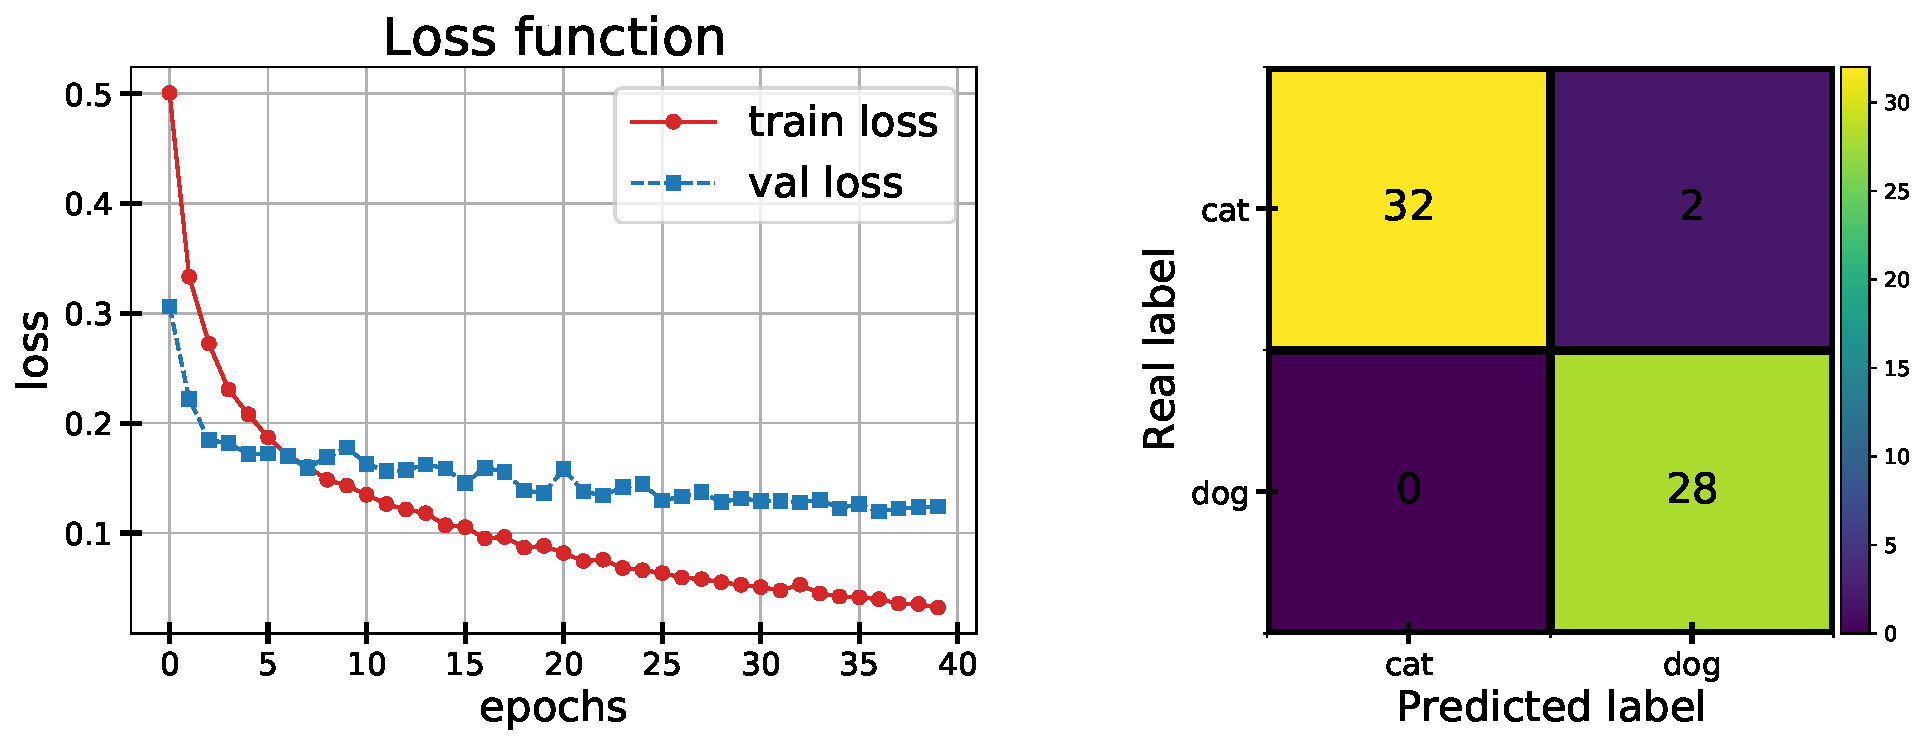
\includegraphics[width=0.8\textwidth]{fig/conf2.pdf}
\caption{The loss as a function of the number of epochs (left) and the confusion matrix of the prediction (right). The test accuracy was 95.16\%.}
\label{fig11}
\end{figure}

\section{Discussion}

In the current project, I managed to prepare and complete a small audio dataset for binary classification. I did preprocess on the dataset to create usable samples. I was looking for commonly used audio features in machine learning. I collected the most proper features for our specific classification task. Then, I used librosa and sklearn to create a dataset consisting of the same finite number of features for all samples.  By applying the learned methods, I created and trained three models (two classical learning and one fully connected neural network model) to classify the test dataset with accuracy higher than 90 percent. The last figure shows the ROC curve of the different classifications and the corresponding AUC scores (see FIG. ~\ref{fig12}).

\begin{figure}[H]
\centering
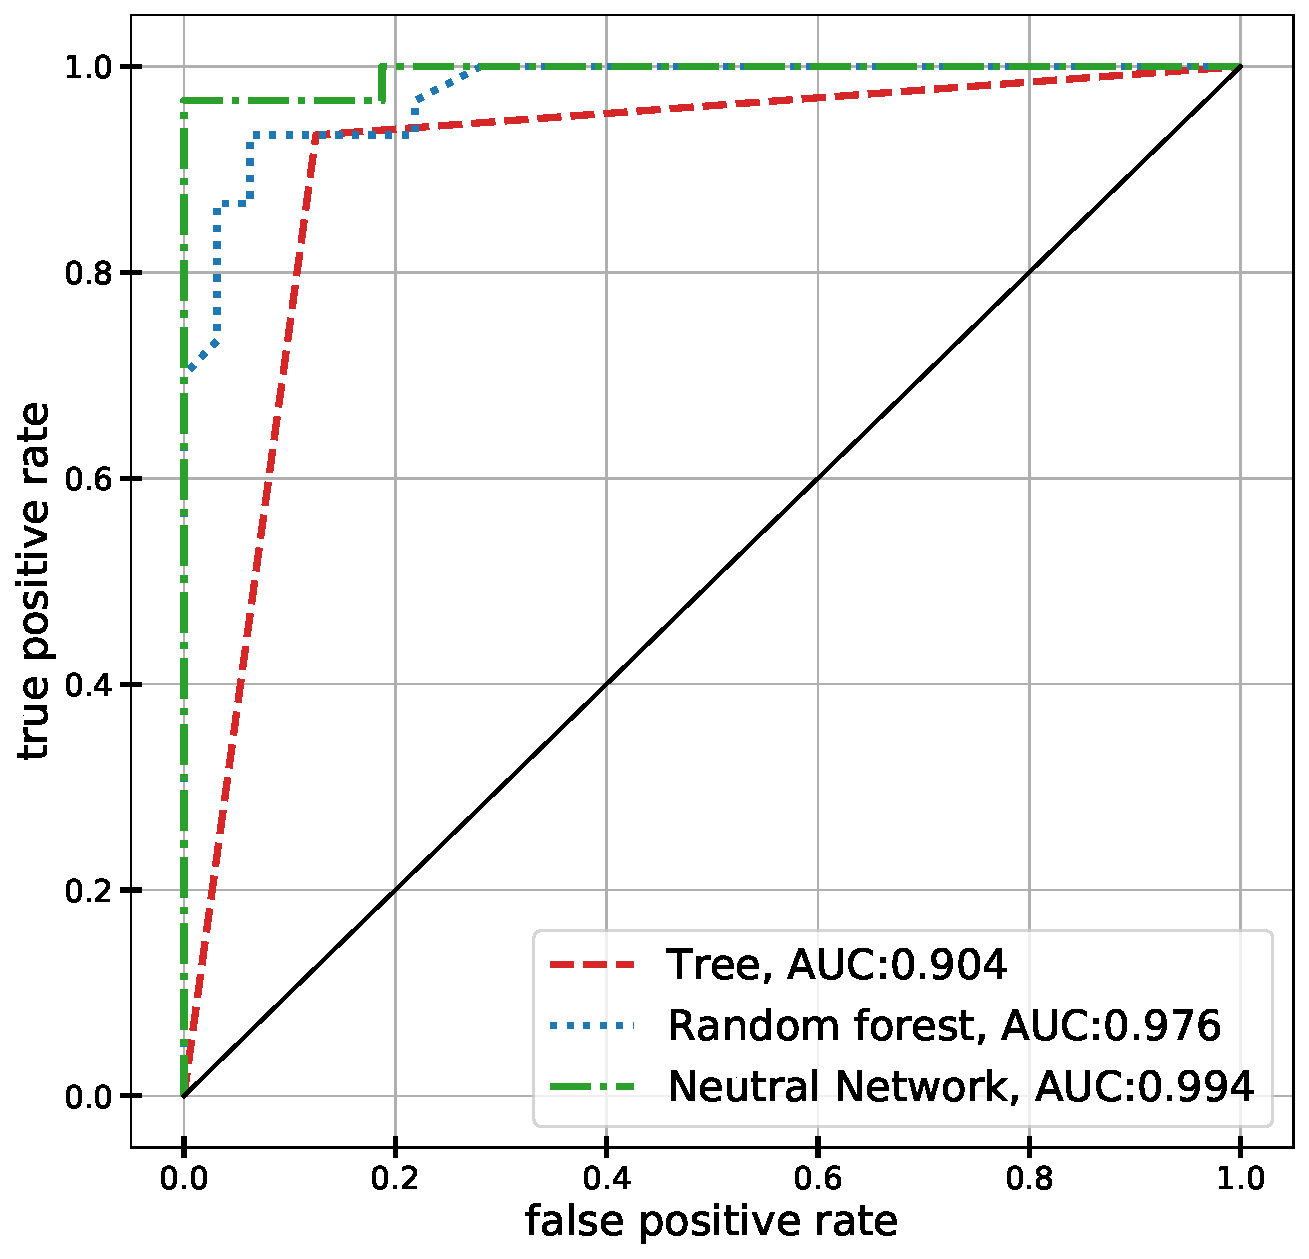
\includegraphics[width=0.6\textwidth]{fig/ROC.pdf}
\caption{The corresponding ROC curves and AUC scores to the three classifier models: decision tree, random forest, fully connected neutral network.}
\label{fig12}
\end{figure}

\begin{thebibliography}{6}
\bibitem{data} \href{https://www.kaggle.com/mmoreaux/audio-cats-and-dogs}{Audio Cats and Dogs}

\bibitem{data2} \href{https://zenodo.org/record/3563990#.YZ99xtDMK3B}{BarkMeowDB - WAV Files of Dogs and Cats}

\bibitem{1} \href{https://www.analyticsvidhya.com/blog/2021/06/introduction-to-audio-classification/}{Introduction to Audio Classification}

\bibitem{2} \href{http://www2.cs.uregina.ca/~gerhard/publications/CAI00.pdf}{David Gerhard, Audio Signal Classification: An Overview}

\bibitem{3} \href{https://devopedia.org/audio-feature-extraction}{Devopedia. 2021. - Audio Feature Extraction.}

\bibitem{repo} \href{https://github.com/portikattila/Data_mining_project}{Data mining project -- GitHub repository}

\end{thebibliography}


\end{document}



